\documentclass[10pt]{article}
\usepackage{amsmath}
\usepackage{amsfonts}
\usepackage{amssymb}
\usepackage{graphicx}
\usepackage{tabularx}
\usepackage[margin=1in]{geometry}
\usepackage[labelfont=bf,labelsep=period]{caption}
\usepackage{booktabs}
\usepackage{multirow}
\usepackage{subcaption}

\title{Monte Carlo as Approximate Polynomial Preconditioning within MCSA}
\author{Steven Hamilton}

\newcommand{\bx}{\ensuremath{\mathbf{x}}}
\newcommand{\by}{\ensuremath{\mathbf{y}}}
\newcommand{\bb}{\ensuremath{\mathbf{b}}}
\newcommand{\bc}{\ensuremath{\mathbf{c}}}
\newcommand{\br}{\ensuremath{\mathbf{r}}}
\newcommand{\bp}{\ensuremath{\mathbf{p}}}
\newcommand{\bw}{\ensuremath{\mathbf{w}}}
\newcommand{\bA}{\ensuremath{\mathbf{A}}}
\newcommand{\bH}{\ensuremath{\mathbf{H}}}
\newcommand{\bM}{\ensuremath{\mathbf{M}}}
\newcommand{\bP}{\ensuremath{\mathbf{P}}}
\newcommand{\bW}{\ensuremath{\mathbf{W}}}
\newcommand{\bI}{\ensuremath{\mathbf{I}}}
\newcommand{\bK}{\ensuremath{\mathbf{K}}}
\newcommand{\calK}{\ensuremath{\mathcal{K}}}

\DeclareMathOperator*{\argmin}{arg\,min}
\newcolumntype{Y}{>{\centering\arraybackslash}X}

\begin{document}
\maketitle

\section{Background}
\label{sec:background}

Monte Carlo Synthetic Acceleration (MCSA), as described in Ref.~\cite{evans_13},
is an approach for solving the linear system
\begin{equation}
\bA \bx = \bb \label{eq:lin_problem}
\end{equation}
using a Monte Carlo (stochastic) process.
The original MCSA algorithm can be written as
\begin{equation}
\begin{aligned}
\bx^{k+1/2} &= \bx^{k} + \br^{k} \\
\bx^{k+1} &= \bx^{k+1/2} + \bM^{-1}\br^{k+1/2} \:,
\end{aligned}
\end{equation}
where $\bM^{-1}$ denotes performing an approximate linear solve using a
Monte Carlo process and $k$ is the iteration index.
Thus, MCSA consists of a single unpreconditioned
Richardson iteration followed by a single preconditioned Richardson iteration.
This iteration scheme has been observed to exhibit far better convergence
behavior than the original sequential Monte Carlo scheme proposed by Halton
\cite{halton_94}.

Both forward (direct) and adjoint Monte Carlo processes have been considered
\cite{slattery_13,evans_13}.
Both approaches work by approximating the Neumann
series of the inverse of \bA:
\begin{equation}
\bA^{-1} = \sum_{n=0}^{\infty} ( \bI - \bA )^n
\equiv \sum_{n=0}^{\infty} \bH^n \:, \label{eq:neumann_inv}
\end{equation}
where \bH\ is the Richardson iteration matrix.
Correspondingly, the solution to a linear system of equations can
be written as
\begin{equation}
\bx = \sum_{n=0}^{\infty} \bH^n \bb \:. \label{eq:neumann_soln}
\end{equation}
Clearly
Eqs.~\eqref{eq:neumann_inv} and \eqref{eq:neumann_soln} are only
valid if the spectral radius of
the iteration matrix, $\rho(\bH)$, is less than unity.

The forward Monte Carlo process is conducted by decomposing the transpose of
\bH\ into an element-wise
(Hadamard) product of a probability matrix and a weight matrix, i.e.
\begin{equation}
\bH = \bP \circ \bW \:. \label{eq:forward_mc_decomp}
\end{equation}
The usual approach is to define rows of \bP\ as normalized rows of \bH\
(normalized columns of \bH), i.e.
\begin{equation}
\bP_{ij} =
\frac{\vert \bH_{ij} \vert}{\displaystyle \sum_{j=1}^{N} \vert \bH_{ij} \vert} \:.
\end{equation}
With this definition for \bP, the weight matrix is given by
\begin{equation}
\bW_{ij} = \frac{\bH_{ij}}{\bP_{ij}}. \label{eq:wgt_mat}
\end{equation}
Note that both \bP\ and \bW\ should have the same sparsity pattern
as $\bH^T$ and so Eq.~\eqref{eq:wgt_mat} is only taken over the indices corresponding
to nonzero entries in $\bH^T$.
A similar process is conducted in the adjoint Monte Carlo process,
except rather than Eq.~\eqref{eq:forward_mc_decomp}, the {\em transpose}
of \bH\ is decomposed, i.e.
\begin{equation}
\bH^T = \bP \circ \bW \:. \label{eq:adjoint_mc_decomp}
\end{equation}
The solution to a system of equations is approximated by following
a number of histories and averaging the contributions
to the solution over all conducted histories.  Histories can be terminated
when the weight decreases by a prescribed fraction (denoted a weight cutoff)
or, alternatively, a history can be terminated after a fixed number of
transitions have taken place (denoted a history length cutoff).

The primary difference
between the forward and adjoint methods is that in the forward method
a contribution is made to the element of the solution vector where the
history originated based on the value of the right hand side in the state
where the history currently resides.  In the adjoint method, however,
a contribution is made to the element of the solution vector where the
history currently resides based on the value of the right hand side
where the history originated.  In the forward method, therefore, it is
necessary to start at least one history in every state in order to
estimate every element of the solution vector whereas in the adjoint
method an estimate of all entries in the solution vector can be
obtained with far fewer than one history per state.
Further details about the Monte Carlo process, including selection
of starting probabilities and different solution tally approaches,
can be found in Ref.~\cite{slattery_13}.

\section{Monte Carlo as Approximate Polynomial Preconditioning}
\label{sec:polynomial_prec}

As described in the previous section, the original idea behind
the adjoint Monte Carlo approach is to approximate the
Neumann series applied to the vector \bb.
However, by applying a history length cutoff it is possible to
view the Monte Carlo random walk as an approximation of a
fixed degree polynomial:
\begin{equation}
p(\bA) = \sum_{n=0}^{m} c_n \left( \bI - \bA \right)^n \:, \label{eq:neumann_poly}
\end{equation}
where in the standard algorithm, $c_n=1$.
The Neumann series is not the only polynomial that can approximate
$\bA^{-1}$, however.  By varying the selection of $c_n$, it is
possible to use other polynomials.  Commonly, polynomials used
for preconditioning are defined in terms of powers of \bA\ rather
than powers of $\bI-\bA$, giving the expansion
\begin{equation}
p(\bA) = \sum_{n=0}^{m} \hat{c}_n \bA^n \:. \label{eq:power_poly}
\end{equation}
Converting between coefficients defined by Eq.~\eqref{eq:power_poly}
and those defined by Eq.~\eqref{eq:neumann_poly} can be
accomplished by means of a change of basis.  It should be denoted
that using $\bI - \bA$ as a basis is generally preferred over using
\bA\ itself.  The reason for this is that if a diagonal scaling
is first applied to \bA, then $\bI-\bA$ will have all zeros
on the main diagonal which eliminates Monte Carlo events in which
a history does not change states.
We now consider several candidates for the matrix polynomial.

\subsection{Chebyshev Polynomials}
\label{subsec:chebyshev}

One approach to defining a preconditioner, $\bM$, is to
attempt to minimize the eigenvalues of $\bI - p(\bA) \bA$.
The Chebyshev polynomials, denoted $T_m(x)$ have the property
that out of all monic polynomials of degree $m$,
$\frac{1}{2^{m-1}} T_m(x)$ is the polynomial whose maximum
absolute value is minimized over the interval $[-1,1]$.
Thus, if the spectrum of \bA is real, then an optimal polynomial
preconditioner can be achieved by mapping the eigenvalues of
\bA\ into the interval $[-1,1]$ using the transformation
\begin{equation}
\ell (\bA) = \alpha \bI + \beta \bA \:,
\end{equation}
where $\alpha  \equiv -\dfrac{\lambda_\text{max} + \lambda_\text{min}}
{\lambda_\text{max} -  \lambda_\text{min}}$,
$\beta \equiv \dfrac{2}{\lambda_\text{max} -  \lambda_\text{min}}$,
and $\lambda_\text{min}$ and $\lambda_\text{max}$ are the
minimum and maximum eigenvalues of $\bA$, respectively.
To see that $\ell(A)$ maps the eigenvalues of $\bA$ into $[-1,1]$,
observe that $\ell(x)$ maps $\lambda_\text{min}$ to -1 and
$\lambda_\text{max}$ to 1.
Then we can select $p(\bA)$ such that
\begin{equation}
\bI - p(\bA) \bA  = \frac{1}{T_{m+1}(\alpha)}
T_{m+1} \left( \ell(\bA) \right) \:, \label{eq:cheby_prec}
\end{equation}
where $\frac{1}{T_m ( \alpha )}$ forces the leading
term of the right hand side to have a coefficient of 1.
To determine an explicit representation for $p(\bA)$, we first
use Eq.~\eqref{eq:power_poly} to write
\begin{equation}
p(\bA) = \sum_{n=0}^{m} c_n \bA^n
\end{equation}
and therefore
\begin{equation}
\bI - p(\bA) \bA = \bI - \sum_{n=0}^{m} c_n \bA^{n+1} \:. \label{eq:poly_prec}
\end{equation}
One possible explicit representation for the Chebyshev polynomial of degree $m$ is
\begin{equation}
T_m(x) = \sum_{n=0}^{\lfloor \frac{m}{2} \rfloor} \left( -1 \right)^n 2^{m - 2n -1} \frac{m}{m-n}
\begin{pmatrix} m-n \\ n \end{pmatrix} x^{m-2n} \:,
\end{equation}
and therefore
\begin{equation}
T_m \left( \ell(\bA) \right) = \sum_{n=0}^{\lfloor \frac{m}{2} \rfloor} \left( -1 \right)^n 2^{m - 2n -1} \frac{m}{m-n}
\begin{pmatrix} m-n \\ n \end{pmatrix} \left( \alpha \bI + \beta \bA \right)^{m-2n} \:.
\end{equation}
Thus an explicit representation for the polynomial preconditioner can
be obtained by equating the right hand sides of Eqs.~\eqref{eq:cheby_prec}
and \eqref{eq:poly_prec}.  For example, using a Chebyshev polynomial of
degree two provides a polynomial preconditioner of degree one described by
\begin{equation}
\begin{aligned}
c_0 &= - \frac{4 \alpha \beta}{2 \alpha^2 -1} \:, \\
c_1 &= - \frac{2 \beta^2}{2 \alpha^2 - 1} \:,
\end{aligned}
\end{equation}
and selecting a Chebyshev polynomial of degree three gives a polynomial
preconditioner of degree two described by
\begin{equation}
\begin{aligned}
c_0 &= - \frac{12 \alpha^2 \beta - 3 \beta}{4 \alpha^3 - 3 \alpha} \:, \\
c_1 &= - \frac{12 \alpha \beta^2}{4 \alpha^3 - 3 \alpha} \:, \\
c_2 &= - \frac{4 \beta^3}{4 \alpha^3 - 3 \alpha} \:.
\end{aligned}
\end{equation}

A significant downside to the use of Chebyshev polynomials is the need for
accurate bounds on the spectrum of $\bA$.  For nonsymmetric matrices,
this requires not only computing smallest and largest eigenvalues as is
required in the symmetric case but requires
bounding the entire spectrum of $\bA$ in an ellipse.  A process for
computing such bounding ellipses is described in Ref.~\cite{manteuffel_77}.

\subsection{GMRES Polynomial}
\label{subsec:gmres_poly}

An alternative class of polynomials requiring less spectral information
than Chebyshev polynomials
while handling nonsymmetric systems naturally is the polynomials generated
by GMRES \cite{saad_86}.  The GMRES algorithm computes, at iteration $m$,
an approximate solution to Eq.~\eqref{eq:lin_problem}, $\bx^{(m)}$,
such that the $L_2$ norm of the residual
is minimized over the $(m+1)$-dimensional Krylov subspace given by
\begin{equation}
\calK_{m+1}(\bA,\bb) = \text{span}\{ \bb, \bA \bb, \ldots, \bA^{m} \bb \}.
\end{equation}
From this definition it is clear that GMRES is constructing (implicitly)
a polynomial of degree $m$, $p_m(\bA)$, such that $p_m(\bA) \approx \bA^{-1}$.
Use of the the GMRES polynomial has been studied as a preconditioner
to fixed point iterations (so-called hybrid GMRES methods)
\cite{elman_86,nachtigal_92,joubert_94}
and as a preconditioner to {GMRES} itself \cite{liu_14}.
Additionally, using the GMRES/Arnoldi process to obtain information about
the matrix for use in a subsequent iterative process has also been
studied \cite{elman_86_2,saylor_90,saylor_91}.

In the context of hybrid GMRES methods, the coefficients of the GMRES polynomial
are generally not computed explicitly, rather the polynomial is applied
to a vector using relationships between the Krylov basis vectors arising from
the Arnoldi process.  In order to use a polynomial within the Monte Carlo
process, however, an explicit representation of the polynomial coefficients
is required.  Multiple approaches for computation of these coefficients
are possible.  One possibility is to observe that the eigenvalues of the
upper Hessenberg matrix generated by the Arnoldi process are the roots of the
GMRES polynomial.  Therefore the polynomial can be written as
\begin{equation}
p_m(x) = \prod_{i=1}^{m} (x - \lambda_i) \:, \label{eq:prod_gmres_poly}
\end{equation}
where $\lambda_i$ are the eigenvalues of the Hessenberg matrix.
Computing the coefficients in the form of Eq.~\eqref{eq:power_poly}
is then simply a matter of expanding the terms in Eq.~\eqref{eq:prod_gmres_poly}.
A second method for computing the GMRES polynomial coefficients arises
directly from the GMRES minimization problem:
\begin{align}
\bx^{(m)} = \argmin_x \Vert \bb - \bA \bx \Vert_2 \\
\text{s.t.} \quad \bx \in \calK_{m+1}(\bA,\bb) \:.
\end{align}
By choosing the ``na\"ive'' basis for the Krylov subspace,
\begin{equation}
\bK_{m+1} = \left[ \bb, \bA \bb, \ldots, \bA^m \bb \right] \:,
\end{equation}
the coefficients of the GMRES polynomial are given by the solution to
the least squares problem
\begin{equation}
\min_{\bc} \Vert \bA \bK_{m+1} \bc - \bb \Vert_2 \:. \label{eq:gmres_min}
\end{equation}
In Ref.~\cite{liu_14}, the surprising observation was made that solving
Eq.~\eqref{eq:gmres_min} using the normal equations actually produced
a more accurate result than using a QR factorization to solve
Eq.~\eqref{eq:gmres_min} or using Eq.~\eqref{eq:prod_gmres_poly}.
Our experience, however, differs from this result.
Figure~\ref{fig:gmres_poly} shows the GMRES polynomial with coefficients
computed using either Eq.~\eqref{eq:prod_gmres_poly} or by
Eq.~\eqref{eq:gmres_min} with two different least squares solvers.
The matrix \bA\ is a $25 \times 25$ 1-D Laplacian with $0.05$ added
to each diagonal entry and the initial vector is taken to be a
normally-distributed random vector.  At a polynomial order of 5,
the two least squares methods are equivalent and appear to perform
significantly better than the Hessenberg eigenvalue approach
(i.e. the magnitude of the polynomials are smaller over the majority
of the region of interest).  At a polynomial order of 10, the behavior
is similar to the $m=5$ case except that a slight difference between the
two least square solutions is now evident.
For orders $15$ and $20$, however, both the eigenvalue-based approach
and the least squares QR perform very well while the normal equations
solution begins to rapidly degrade.
Table~\ref{tab:gmres_poly} shows the value
of the spectral radius of $\bI - p_m(\bA) \bA$ for each
of these cases.  Both the eigenvalue approach and the least squares QR
produce monotonically decreasing spectral radii whereas the spectral
radius produced by the normal equations increases at high polynomial
orders.  The least squares QR method seems to produce the most consistent
behavior over the full range of polynomial orders.
The significant variability in the different methods for computing the
coefficients of the GMRES polynomial are indicative of the ill-conditioned
nature of computations involving polynomial coefficients.
\begin{figure}
\centering
\begin{subfigure}[b]{0.49\linewidth}
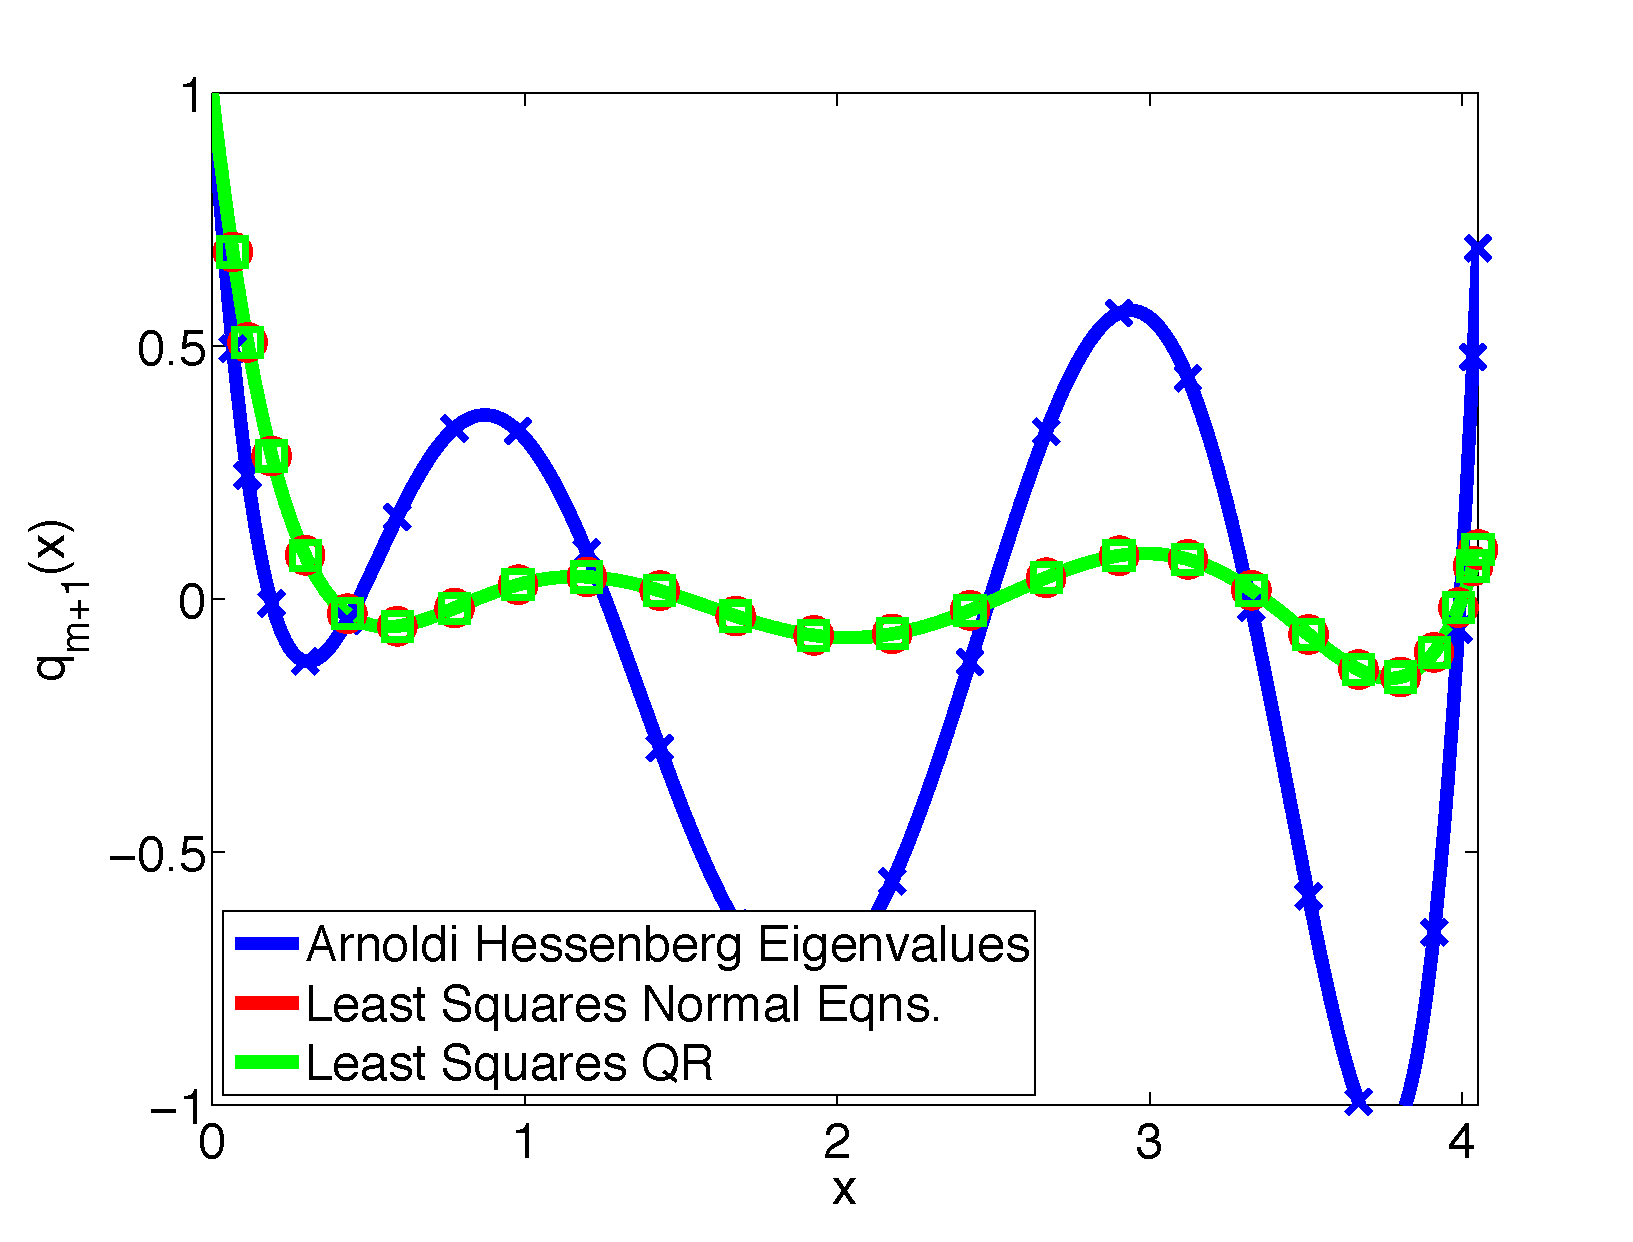
\includegraphics[width=\textwidth]{gmres_poly5}
\caption{$m = 5$}
\end{subfigure}
\begin{subfigure}[b]{0.49\linewidth}
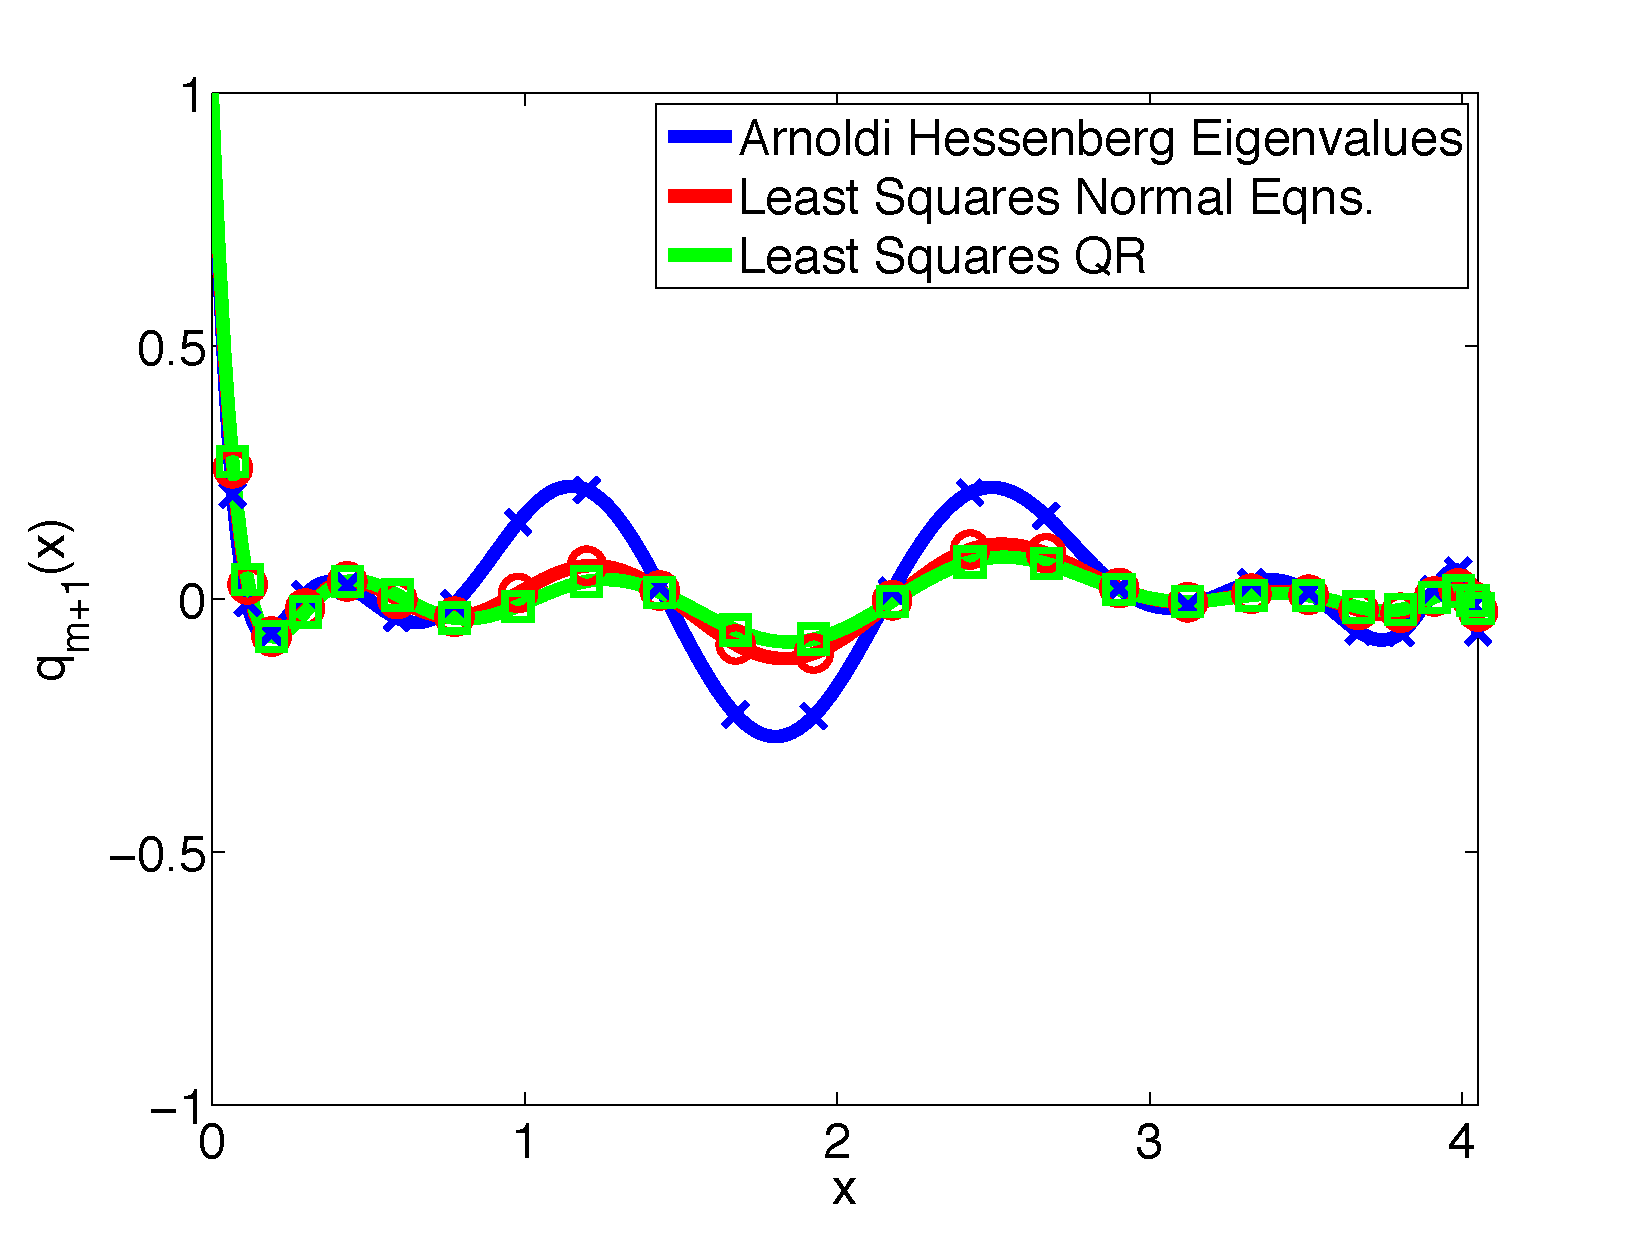
\includegraphics[width=\textwidth]{gmres_poly10}
\caption{$m = 10$}
\end{subfigure}
\begin{subfigure}[b]{0.49\linewidth}
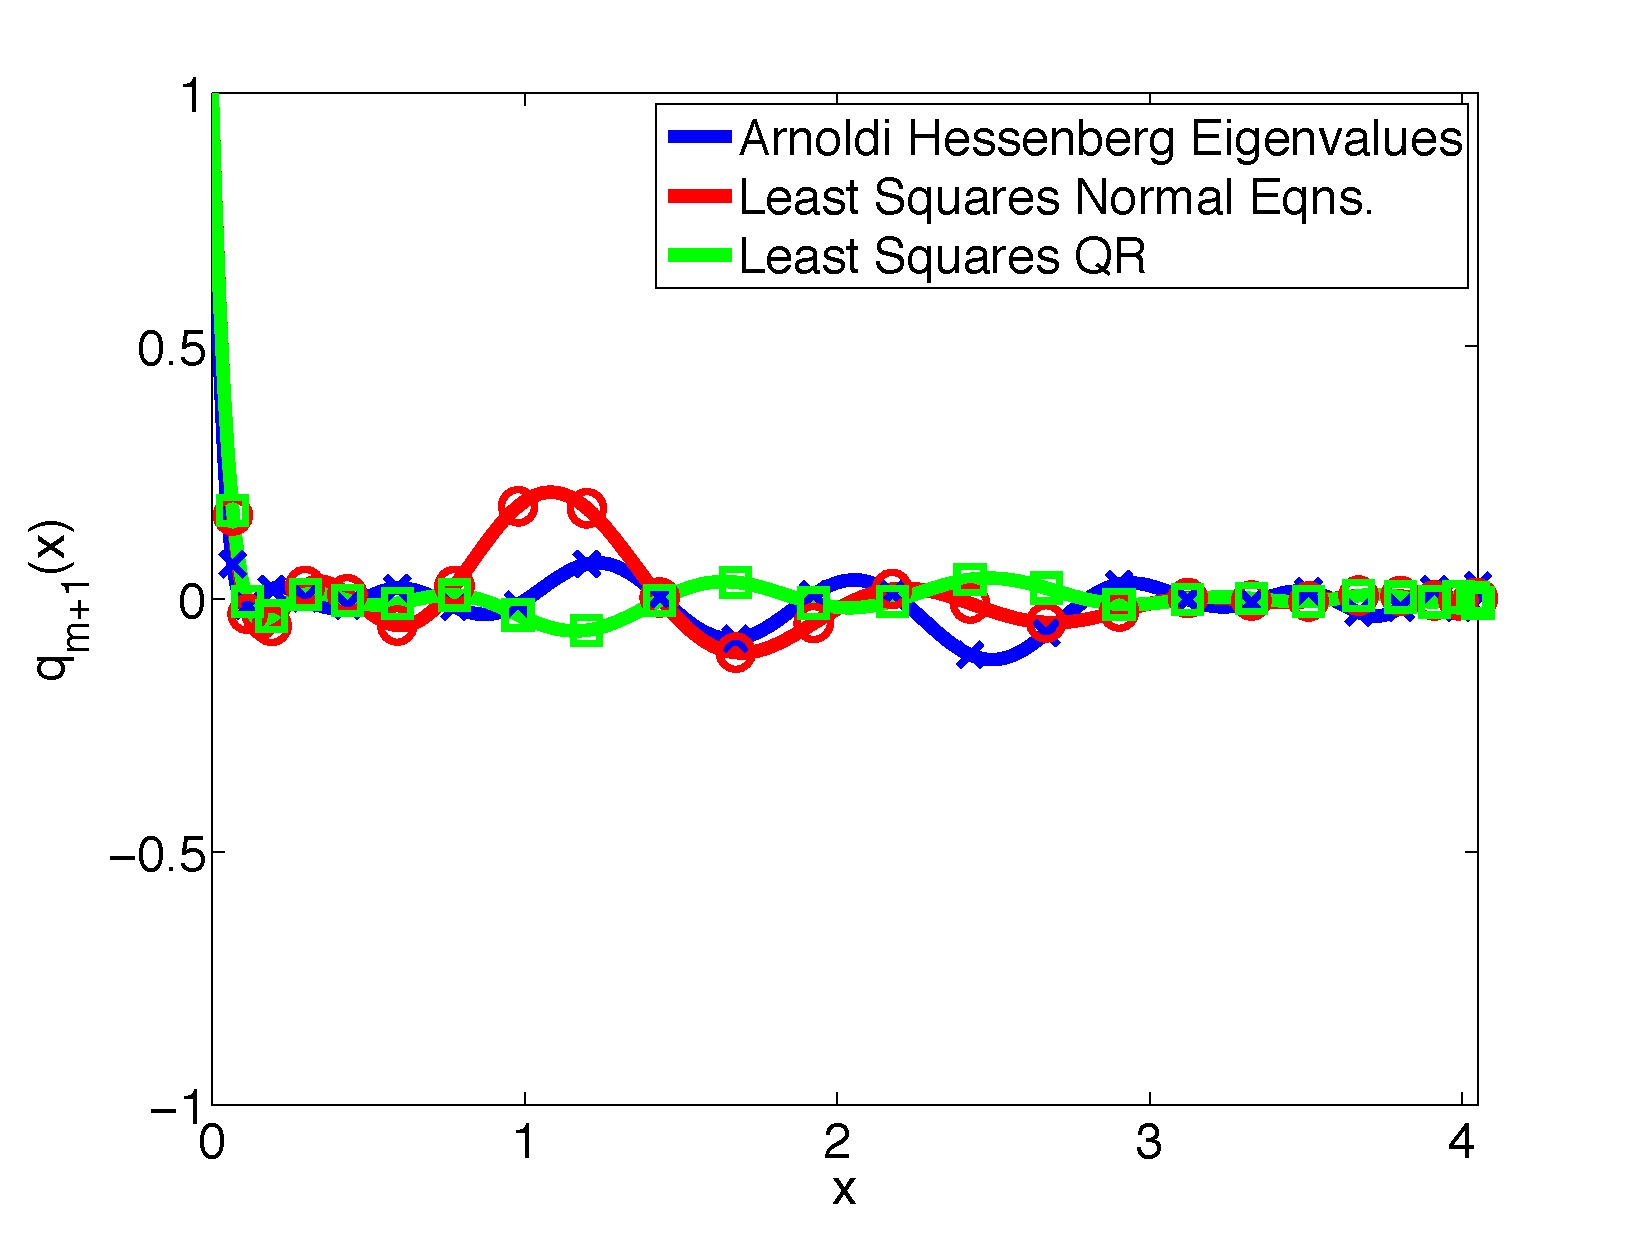
\includegraphics[width=\textwidth]{gmres_poly15}
\caption{$m = 15$}
\end{subfigure}
\begin{subfigure}[b]{0.49\linewidth}
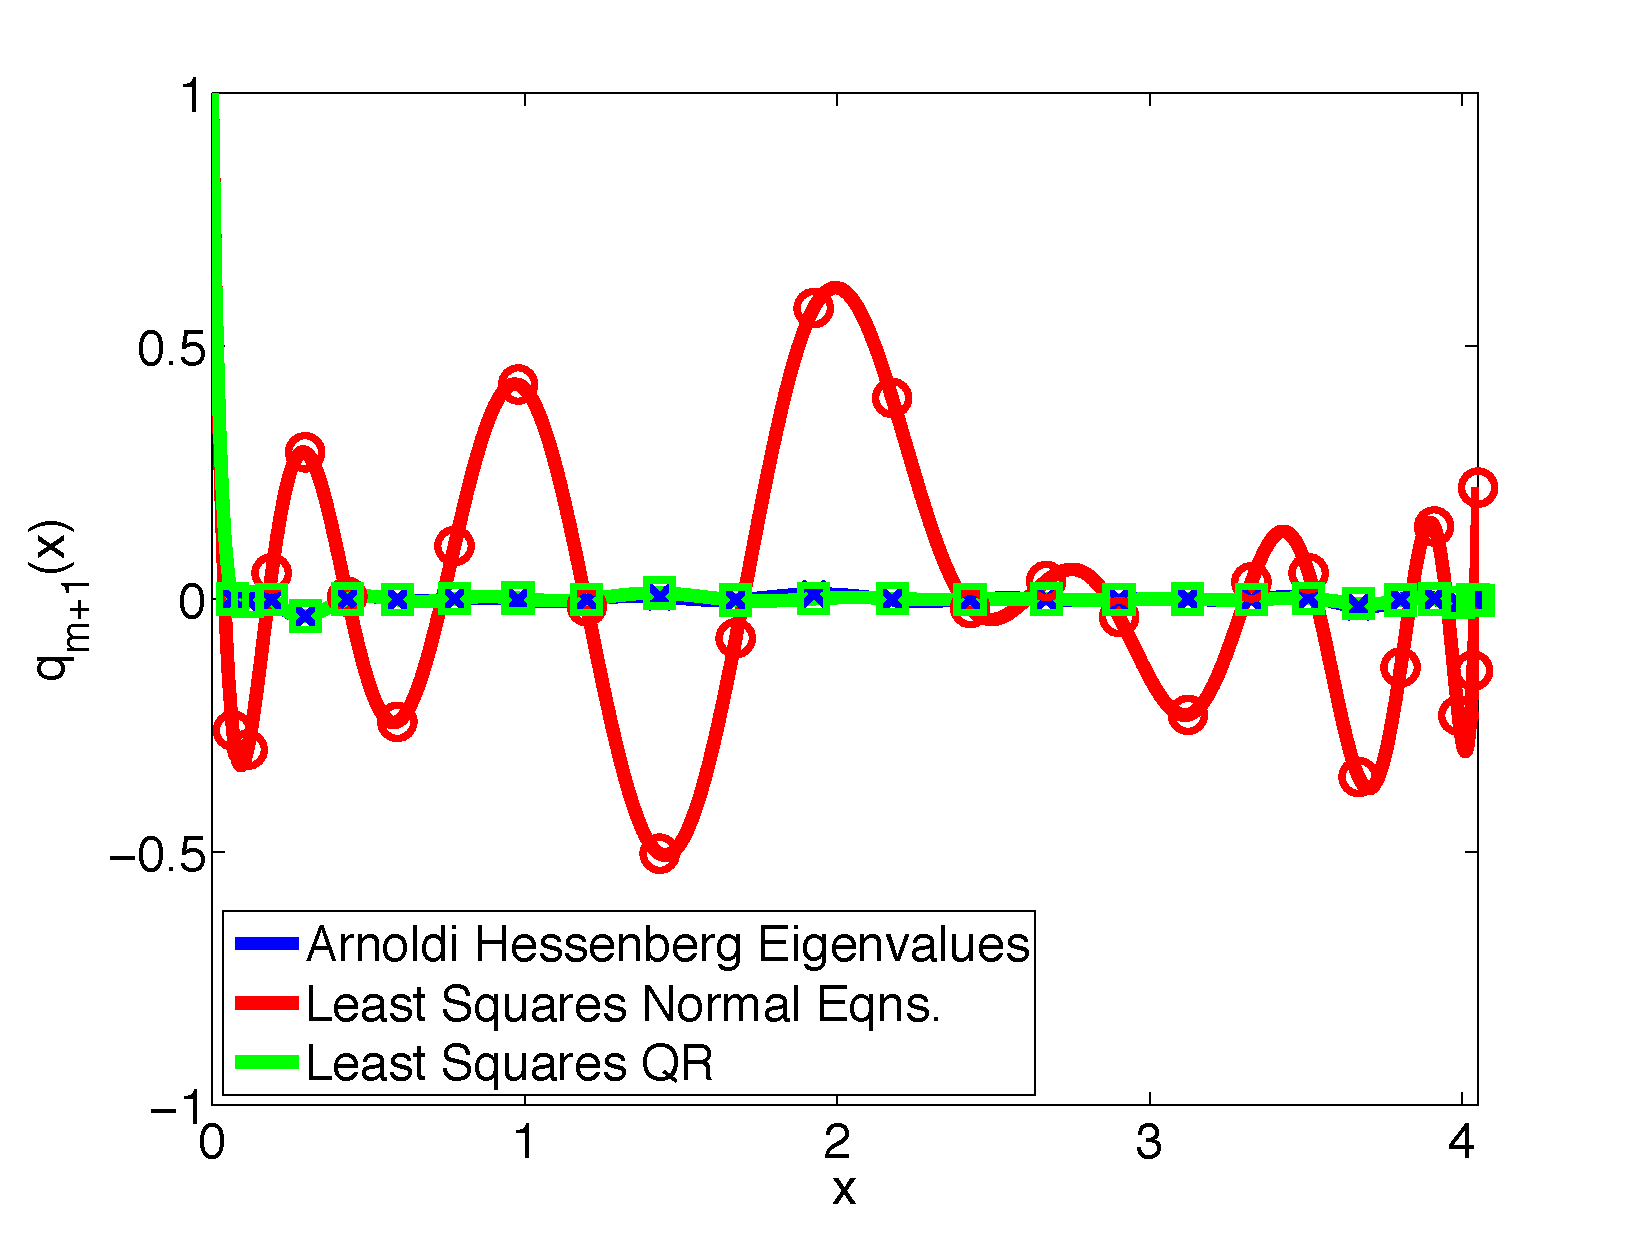
\includegraphics[width=\textwidth]{gmres_poly20}
\caption{$m = 20$}
\end{subfigure}
\caption{Plot of $q_{m+1}(x)=1-xp_{m}(x)$, where $p_m(x)$ is the GMRES
 polynomial with different methods for computing the coefficients.
 \bA\ is a shifted Laplacian with $N=25$.  Markers
 indicate the polynomials evaluated at the eigenvalues of \bA.}
\label{fig:gmres_poly}
\end{figure}
\begin{table}
\centering
\caption{Spectral Radius of $\left( \bI - p_m(\bA) \bA \right)$.}
\label{tab:gmres_poly}
\begin{tabular}{ccccc}
\toprule
& \multicolumn{4}{c}{Polynomial Order} \\
\cmidrule(r){2-5}
Method & 5 & 10 & 15 & 20 \\
\midrule
Hessenberg Eigenvalues     & 1.027 & 0.630 & 0.081 & 0.034 \\
Least Squares Normal Eqns. & 0.686 & 0.268 & 0.162 & 0.575 \\
Least Squares QR           & 0.686 & 0.281 & 0.085 & 0.033 \\
\bottomrule
\end{tabular}
\end{table}

A significant advantage of GMRES polynomials over Chebyshev is that
GMRES polynomials handle nonsymmetric matrices with potentially complex
eigenvalue naturally, whereas computing the coefficients of
Chebyshev polynomials requires the costly task of bounding the spectrum
of \bA\ in an ellipse.  Additionally, accurate knowledge of the bounding eigenvalues
of \bA\ are required to compute the Chebyshev coefficients of any order
(which may incur a cost of tens or hundreds of matrix-vector products),
while the computation of GMRES polynomial coefficients requires only
$m$ matrix-vector products for an order $m$ polynomial.

\section{Results}
\label{sec:results}

Tables~\ref{tab:lap_forward_neumann} and \ref{tab:lap_adjoint_neumann}
show the behavior of
the standard MCSA algorithm (with forward and adjoint Monte Carlo, respectively)
applied to a $1000 \times 1000$ shifted Laplacian matrix with a shift
of $0.01$.  The right hand side is given by $\bb_i = \sin \left( \pi \frac{i-1}{N-1} \right)$
and the stopping criterion is a reduction in the L$_2$ norm of the residual
by six orders of magnitude.
The effect of varying the polynomial order and the number of Monte Carlo
histories per iteration is shown.
As expected, increasing the polynomial order generally leads to a decrease
in the number of iterations required for convergence.
For a fixed number of histories, however, there is a threshold beyond
which an increase in the polynomial order actually leads to very slow
convergence or even divergence.  Conversely, for a fixed polynomial order
it is necessary to track ``enough'' histories to ensure stability, but
beyond that point there is little benefit to executing additional histories.
Comparing the results for the forward and adjoint methods, the adjoint method
generally requires fewer histories to achieve a stable result.  When both
methods converge, however, the forward method generally achieves convergence
in fewer MCSA iterations.  At low history counts, the adjoint method displays
greater stability for even order polynomials than for add orders, the reason
for this behavior is not clear.
\begin{table}
\caption{Forward MCSA with Neumann Polynomial, $1000 \times 1000$ Shifted Laplacian Matrix.
Values are MCSA iteration counts (timing in milliseconds)
\label{tab:lap_forward_neumann}}
\centering
\begin{tabularx}{0.8\textwidth}{c *{6}{Y}}
\toprule
Histories per & \multicolumn{6}{c}{Polynomial Order} \\
\cmidrule(lr){2-7}
Iteration & 1 & 2 & 3 & 4 & 5 & 6 \\
\midrule
250 & - & - & - & - & - & - \\
500 & - & - & - & - & - & - \\
1000 & - & - & - & - & - & - \\
2000 & - & - & - & - & - & - \\
4000 & - & 765(249) & 605(285) & 947(560) & 396(302) & 560(458) \\
8000 & 923(325) & 698(413) & 554(485) & 471(560) & 396(530) & 354(561) \\
16000 & 923(616) & 695(809) & 554(946) & 463(1015) & 396(1068) & 348(1079) \\
\bottomrule
\end{tabularx}
\end{table}
\begin{table}
\caption{Adjoint MCSA with Neumann Polynomial, $1000 \times 1000$ Shifted Laplacian Matrix.
Values are MCSA iteration counts (timing in milliseconds)
\label{tab:lap_adjoint_neumann}}
\centering
\begin{tabularx}{0.8\textwidth}{c *{6}{Y}}
\toprule
Histories per & \multicolumn{6}{c}{Polynomial Order} \\
\cmidrule(lr){2-7}
Iteration & 1 & 2 & 3 & 4 & 5 & 6 \\
\midrule
250 & - & 775(100) & - & 651(96) & - & 664(110) \\
500 & - & 725(122) & - & 502(104) & - & 394(95) \\
1000 & - & 707(174) & - & 482(179) & - & 366(144) \\
2000 & 2096(521) & 703(280) & 1991(855) & 471(259) & 2668(1514) & 356(251) \\
4000 & 1694(821) & 698(494) & 1701(1194) & 467(497) & 864(921) & 350(458) \\
8000 & 1384(1142) & 697(923) & 1256(1761) & 464(905) & 628(1290) & 350(873) \\
16000 & 1220(1969) & 695(1796) & 859(2493) & 462(1768) & 588(2384) & 347(1711) \\
\bottomrule
\end{tabularx}
\end{table}

Tables~\ref{tab:lap_forward_cheby} and \ref{tab:lap_adjoint_cheby}
show the same problem using Chebyshev polynomials instead of the Neumann
series polynomial.  Stability seems to be a much greater concern when using
Chebyshev polynomials, as significantly more histories must be executed to
achieve convergence as compared to the corresponding Neumann series results.
One possible explanation for this behavior is that the Chebyshev coefficients
increase exponentially in magnitude, making approximation of higher order terms
far more difficult.
When convergence is achieved, however, significantly smaller iteration counts
are observed.  As with the Neumann series polynomial, greater stability is
achieved when using the adjoint method.
\begin{table}
\caption{Forward MCSA with Chebyshev Polynomial, $1000 \times 1000$ Shifted Laplacian Matrix.
Values are MCSA iteration counts (timing in milliseconds)
\label{tab:lap_forward_cheby}}
\centering
\begin{tabularx}{0.8\textwidth}{c *{6}{Y}}
\toprule
Histories per & \multicolumn{6}{c}{Polynomial Order} \\
\cmidrule(lr){2-7}
Iteration & 1 & 2 & 3 & 4 & 5 & 6 \\
\midrule
250 & - & - & - & - & - & - \\
500 & - & - & - & - & - & - \\
1000 & - & - & - & - & - & - \\
2000 & - & - & - & - & - & - \\
4000 & - & - & - & - & - & - \\
8000 & 556(198) & - & - & - & - & - \\
16000 & 556(363) & - & - & - & - & - \\
\bottomrule
\end{tabularx}
\end{table}
\begin{table}
\caption{Adjoint MCSA with Chebyshev Polynomial, $1000 \times 1000$ Shifted Laplacian Matrix.
Values are MCSA iteration counts (timing in milliseconds)
\label{tab:lap_adjoint_cheby}}
\centering
\begin{tabularx}{0.8\textwidth}{c *{6}{Y}}
\toprule
Histories per & \multicolumn{6}{c}{Polynomial Order} \\
\cmidrule(lr){2-7}
Iteration & 1 & 2 & 3 & 4 & 5 & 6 \\
\midrule
250 & - & - & - & - & - & - \\
500 & - & - & - & - & - & - \\
1000 & - & - & - & - & - & - \\
2000 & - & 328(134) & - & - & - & - \\
4000 & - & 296(210) & - & - & - & - \\
8000 & - & 288(380) & 262(423) & - & - & - \\
16000 & 1132(1866) & 283(721) & 175(550) & - & - & - \\
\bottomrule
\end{tabularx}
\end{table}

Tables~\ref{tab:lap_forward_gmres} and \ref{tab:lap_adjoint_gmres}
again show the results of MCSA applied to the same problem,
now using the GMRES polynomial (computing using the least squares
QR solution described in Section~\ref{subsec:gmres_poly} with a random
initial vector).  The GMRES polynomial seems to offer a favorable
middle ground between the Neumann series and Chebyshev polynomials:
iteration counts for a given polynomial order are smaller than with
the Neumann series and yet far fewer histories are required to achieve
stability than with the Chebyshev polynomial.
\begin{table}
\caption{Forward MCSA with GMRES Polynomial, $1000 \times 1000$ Shifted Laplacian Matrix.
Values are MCSA iteration counts (timing in milliseconds)
\label{tab:lap_forward_gmres}}
\centering
\begin{tabularx}{0.8\textwidth}{c *{6}{Y}}
\toprule
Histories per & \multicolumn{6}{c}{Polynomial Order} \\
\cmidrule(lr){2-7}
Iteration & 1 & 2 & 3 & 4 & 5 & 6 \\
\midrule
250 & - & - & - & - & - & - \\
500 & - & - & - & - & - & - \\
1000 & 923(89) & - & - & - & - & - \\
2000 & 923(127) & 547(110) & - & - & - & - \\
4000 & 923(195) & 547(204) & - & - & - & - \\
8000 & 923(330) & 547(322) & 357(312) & - & - & - \\
16000 & 923(607) & 547(640) & 357(607) & 246(536) & - & - \\
\bottomrule
\end{tabularx}
\end{table}
\begin{table}
\caption{Adjoint MCSA with GMRES Polynomial, $1000 \times 1000$ Shifted Laplacian Matrix.
Values are MCSA iteration counts (timing in milliseconds)
\label{tab:lap_adjoint_gmres}}
\centering
\begin{tabularx}{0.8\textwidth}{c *{6}{Y}}
\toprule
Histories per & \multicolumn{6}{c}{Polynomial Order} \\
\cmidrule(lr){2-7}
Iteration & 1 & 2 & 3 & 4 & 5 & 6 \\
\midrule
250 & 1153(136) & 2572(337) & - & - & - & - \\
500 & 1003(151) & 616(105) & 462(87) & - & - & - \\
1000 & 946(226) & 566(142) & 385(110) & 496(161) & - & - \\
2000 & 933(306) & 557(222) & 368(175) & 260(146) & - & - \\
4000 & 928(519) & 554(412) & 362(311) & 254(259) & 203(236) & - \\
8000 & 924(971) & 549(731) & 362(585) & 251(490) & 184(423) & - \\
16000 & 923(1816) & 548(1426) & 360(1135) & 247(965) & 179(797) & 146(744) \\
\bottomrule
\end{tabularx}
\end{table}

\bibliographystyle{plain}
\bibliography{references}

\end{document}
